\lstset{frameround=fttt,captionpos=b}

\begin{quotation} {\em 
\noindent
The child receives data through the sense organs; the child also has
some inborn processing capacities~-- otherwise it would not be able
to learn~-- but in addition, some ``information'' or ``programs'' are
built-in at birth
%(for example, the child does not have to learn how to suck, for this
%is an innate reflex); 
\ldots
there is a working memory
%, in which the child keeps those items of knowledge that are being
%used at a particular moment;
\ldots
and there is a permanent memory
%, which is, in Locke's terms, largely a ``blank tablet'' at birth, but
%which has a storage capacity that makes a hard disk pale into
%insignificance.  The child gradually builds up a symbolic
%representation of the world around it, 
\ldots
so there must be some inner ``language'' or medium of representation
%; even a newborn baby is starting to see and taste and smell and hear
%and touch, and to remember the more striking of its experiences, so
%the internal medium by which it represents and stores these
%impressions cannot be the native language (of which it is still
%ignorant. 
\ldots 
Jerry Fodor
%[in The Language of Thought]
\ldots
has discussed this inbuilt ``language of thought,'' which is similar
conceptually to the ``machine language'' that is built into the
personal computer.
%and about which most users remain completely ignorant).
}

-- John Cleverly, in ``Visions of childhood: Influential models from
Locke to Spock'' \cite{cleverley1986visions}
\end{quotation}


\section{Introduction}

{\bf Machine language}, or {\bf machine code}, is the set of
instructions that a computer's central processing unit (CPU)
understands.  It is the binary 0's and 1's that form instructions for
the CPU to execute.  When we compile a program, that program is
eventually converted to binary machine code, which we can then run.
Each different CPU has a different machine language that it
understands, although CPU families tend to understand a very similar
language.

Programming in machine language requires one to write the code in
hexadecimal notation, manually encoding the instructions one at a
time.  For this reason, machine language can often be difficult to
program in.  This is especially true with the complexities of modern
instruction sets on processor families such as the x86 and MIPS.

One will often write a program in {\bf assembly language}, which is a
(somewhat) higher-level manner to create a program.  In assembly
language, one can specify to add two values together through a command
such as {\tt sub esp, 24}, and need not write it in the hexadecimal
notation of 0x83ec20.
% to get that value, compile test_abs_c.c via: 'g++ -m32 -o test_abs_c
% test_abs_c.c', load it into gdb, and run 'disassemble /r main'.
% It's the 4th line (or so) of the main function.
An {\bf assembler} is a program that converts assembly language into
machine language.  In fact, compilers typically produce assembly
language, and then call the assembler to produce the machine code.

Learning how machine language works allows us to truly understand how
a machine operates at a very low level.

In this chapter we introduce a simplified machine language called the
Itty Bitty Computing Machine, or IBCM.  This machine language is
designed to be simple enough that it can be learned in a reasonable
amount of time, but complex enough that one can use it to write a wide
range of programs.  It is intended to teach many of the important
concepts of a modern machine language without having to deal with the
complexities of~-- and time required to learn~-- modern CPU machine
languages.


\section{Memory Hierarchy}

Typically, computer programs do not differentiate between the various
levels of memory.  Programs tend to view memory as a monolithic whole,
and allocate memory as needed.  In fact, there are many different
levels of memory.  Fast memory~-- formally called {\em static
  random-access memory} or SRAM~-- is expensive to make, and computers
would be quite expensive if all memory were fast memory.  In fact,
some super computers did just this~-- the Cray Y-MP, a super computer
from the late 1980's, used only SRAM, and it cost approximately 10
million dollars.
% http://en.wikipedia.org/wiki/Cray_Y-MP
% cost: http://www.geek.com/articles/news/cray-for-sale-on-ebay-2000097/

Instead, most computers use primarily {dynamic random-access memory},
or DRAM, as the primary component of main memory, and use a smaller
amount of SRAM to speed up computations.  SRAM is used in the {\em
  cache}, although we will not go into detail about caches here.

\begin{wrapfigure}{r}{0.55\textwidth}
\begin{center}
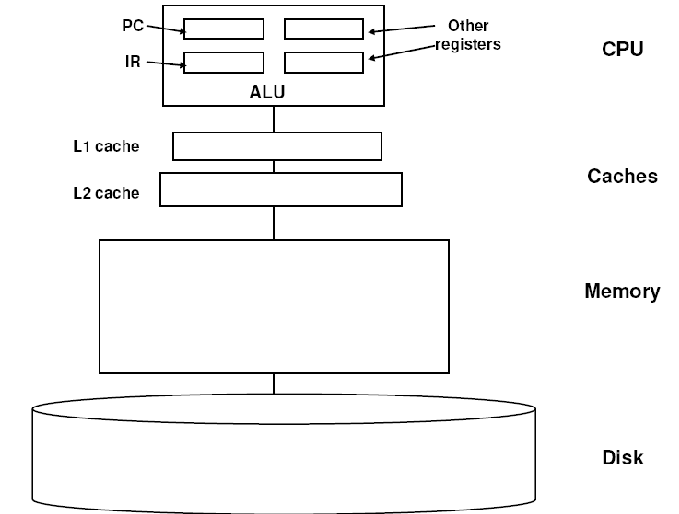
\includegraphics[width=4in]{ibcm/memory-hierarchy.png}
\end{center}
\caption{Memory Hierarchy}
\label{memory-hierarchy}
\vspace{-0.6in}
\end{wrapfigure}

The four primary levels of memory are listed below.  Cost decreases
and storage capacity increases as one moves down the list.

\begin{itemlist}
\item CPU registers
\item Static random-access memory (SRAM) in various levels of cache
  (L1 cache, L2 cache, etc.)
\item Dynamic random-access memory (DRAM) used in main memory
\item Hard drive storage, either on a traditional hard disk with
  rotating platters, or on solid state hardware.
\end{itemlist}

This chapter will largely ignore storing data in cache or on the hard
drive, as that is typically managed by the operating system.  Instead,
we will primarily focus on the values kept in the registers in a CPU,
and in main memory.

Main memory is relatively slow, compared with the speed of a CPU.  In
addition, many CPUs can only allow one memory access per instruction.
Thus, the other values must be kept in a location that is not main memory:
the CPU's registers.  A register is a small area of memory in the CPU
where intermediate computation values can be stored.  A modern CPU
will have registers that each are 32 or 64 bits in size, and may have
12-32 of these registers.

Thus, there are instructions~-- in both machine language and assembly
language~-- that move data between the CPU's registers and main memory.
We will see these instructions shortly.



\section{IBCM Principles of Operation}

\subsection{Machine Description}

The Itty Bitty Computing Machine (IBCM) is a very simple computer.  In
fact, it's so simple that no one in their right mind would build it
using today's technology. Nevertheless~-- except for limits on problem
size~-- any computation that can be performed on the most modern,
sophisticated computer can also be performed on the IBCM.  Its main
virtues are that it can be taught quickly and provides context for
talking about more recent architectures.

The IBCM contains a single register, called the accumulator.  Most
early computers had just an accumulator, and many current
micro-controllers are still accumulator machines.  IBCM's accumulator
can hold a 16-bit 2's complement integer.  In addition, the IBCM has
two other registers: the instruction register (IR), which contains the
current instruction being executed, and the program counter (PC),
which contains the address of the next instruction to be executed.
However, we will not directly use those two registers.

The IBCM has 4,096 addressable memory locations, each one which
location holds a 2 byte (16 bit).  Thus, the IBCM technically has
8,192 bytes (8 Kb) of memory.

The IBCM handles input by reading in single values (either a
hexadecimal value or an ASCII character) into the accumulator.
Similarly, output is handled by writing the value in the accumulator
as either a hexadecimal value or an ASCII character.

\subsection{Instructions}

The IBCM equivalent of ``statements'' in a higher level language are
very simple instructions.  Each instruction is encoded in a 16-bit
word in one of the formats shown in
Figure~\ref{IBCMInstructionFormat}.  Shaded areas in the figure
represent portions of the instruction word whose value does not
matter. For example, a word whose leftmost four bits are zero is an
instruction to halt the computer.


\begin{figure}[h!]
\centering
%\begin{tabular}{cccccccccc}
\begin{tabular}{cccccp{1mm}p{1mm}ccr|lc}

bit: & 15 & 14 & 13 & 12 & 11 & 10 & \ldots &  & \multicolumn{1}{r}{0} & \\
\cline{2-10}

& \multicolumn{1}{|c}{0} & 0 & 0 & \multicolumn{1}{c|}{0} &
\cellcolor[gray]{0.8} & \cellcolor[gray]{0.8} &
(unused)\hspace{0.25in}\cellcolor[gray]{0.8}&\cellcolor[gray]{0.8} &
\cellcolor[gray]{0.8} 
& halt & \multicolumn{1}{c}{\begin{tabular}{c}\\\\\end{tabular}} \\
\cline{2-10}

& \multicolumn{1}{|c}{0} & 0 & 0 & \multicolumn{1}{c|}{1} &
\multicolumn{2}{p{2mm}|}{\begin{tabular}{l}\hspace{-0.075in}I/O\\\hspace{-0.025in}op\\\end{tabular}}
& (unused) \cellcolor[gray]{0.8}& \cellcolor[gray]{0.8} &
\cellcolor[gray]{0.8} & I/O & \\ \cline{2-10}

& \multicolumn{1}{|c}{0} & 0 & 1 & \multicolumn{1}{c|}{0} &
\multicolumn{2}{p{2mm}|}{\begin{tabular}{l}\hspace{-0.09in}shift\\\hspace{-0.025in}op\\\end{tabular}}
& \hspace{0.25in}(unused)\hspace{0.25in} \cellcolor[gray]{0.8}&
\multicolumn{2}{|c|}{count} & shifts & \\ \cline{2-10}

& \multicolumn{4}{|c|}{opcode} & \begin{tabular}{cc}\\\\\end{tabular} &
& address & & & others & \\ \cline{2-10}

\end{tabular}
\caption{IBCM instruction format}
\label{IBCMInstructionFormat}
\end{figure}

A note on using hexadecimal notation: IBCM is a binary computer.
Internally all operations are performed on 16-bit binary values.
However, because it's so tedious and error-prone for humans to write
or read 16-bit quantities, all of IBCM's input/output is done either
as ASCII characters or 4-digit hexadecimal numbers.  Remember that
these are just external shorthands for the internal 16-bit values!

Also, hexadecimal values are often prefixed by a '0x', such as
'0x1234'.

\subsubsection{Halt}
Any instruction where the opcode is zero (i.e., the first 4 bits are
all zero) will halt the IBCM.  It does not matter what the remaining
12 bits are.  Not much else to say on this one.

\subsubsection{Input and Output}

The input and output (or 'I/O') instructions move data between the
accumulator and the computer 'devices'~-- the keyboard and screen.
Data can be moved either as hexadecimal numbers or as an ASCII
character; in the later case, only the bottom (least significant) 8
bits of the accumulator are involved. The next two bits after the
opcode specify if the instruction is an input or output, and if it
will use hexadecimal values or ASCII characters.  The four
possibilities (in/out, hex/ASCII) that are specified by the bits 11 and
10 of the instruction word as shown in
Table~\ref{IBCM-io-instruction-values.tbl}.  Being as there are only
four possibilities, the full hexadecimal encoding of each of the four
I/O instructions is also listed.

\begin{table}[h]
\centering
\begin{tabular}{ccclcl}
\und{bit 11} & \und{bit 10} & & \und{operation} & & \und{hex value} \\
0 & 0 & & read a hexadecimal word (four digits) into the accumulator &
& 0x1000 \\
0 & 1 & & read an ASCII character into the accumulator bits 8-15 & &
0x1400 \\
1 & 0 & & write a hexadecimal word (four digits) from the accumulator
& & 0x1800 \\
1 & 1 & & write an ASCII character from the accumulator bits 8-15 & &
0x1c00 \\
\end{tabular}
\caption{IBCM input/output bit values}
\label{IBCM-io-instruction-values.tbl}
\end{table}

\subsubsection{Shifts and Rotates}

Shifting and rotating are common operations in computers. Shifting
means moving data to the right or left; rotating is much the same
thing except that bits that ``fall off'' one end are reinserted at the
other end.  

The examples below assume that the value being rotated is one byte (8
bits) in length. In reality, the IBCM performs shifts and rotates on
the 16 bit value in the accumulator.  We choose to describe these
operations with 8 bit quantities to make the explanation easier to
understand.

Diagrammatically, a ``right shift'' of ``$n$ positions'' looks like
Figure~\ref{ibcm-shift-1} when $n = 3$:

\begin{figure}[h]
\centering
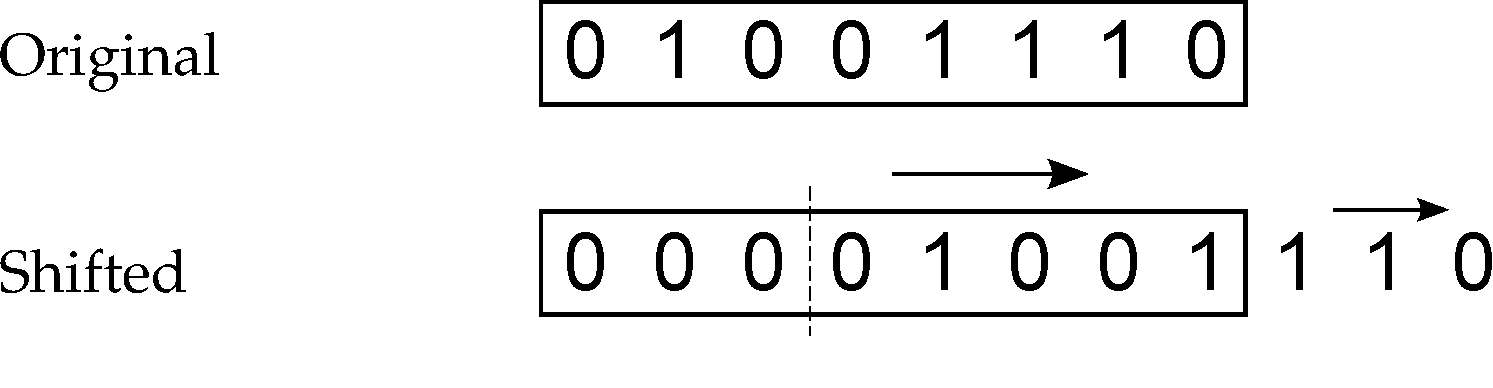
\includegraphics[width=4in]{ibcm/ibcm-shift-1.pdf}
\caption{A right shift of 3}
\label{ibcm-shift-1}
\end{figure}

Each bit is moved $n$ positions to the right (three in this case).
Alternatively, it is moved one bit to the right $n$ times. This causes
the original $n$ right-most bits to fall off the right end and $n$ new
(zero) bits to be inserted at the left end. A ``left shift'' is much
the same, except that bits move to the left, as shown in
Figure~\ref{ibcm-shift-2}.

\begin{figure}[h]
\centering
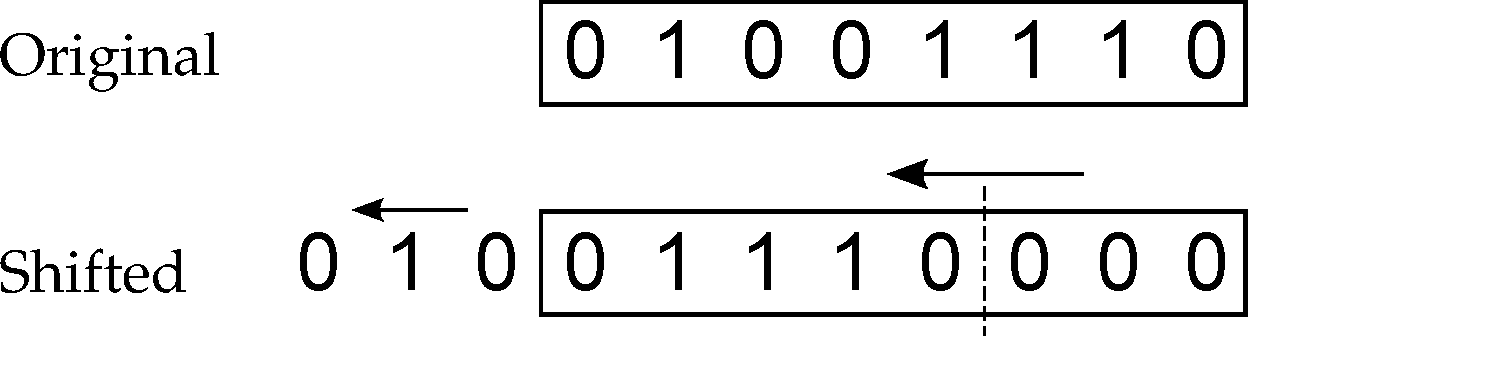
\includegraphics[width=4in]{ibcm/ibcm-shift-2.pdf}
\caption{A left shift of 3}
\label{ibcm-shift-2}
\end{figure}

As noted previously, rotates are like shifts except that the bits that
fall off one end but are reinserted at the other end.
Figure~\ref{ibcm-shift-3} is a left rotation; right rotates are left
to your imagination.

\begin{figure}[h]
\centering
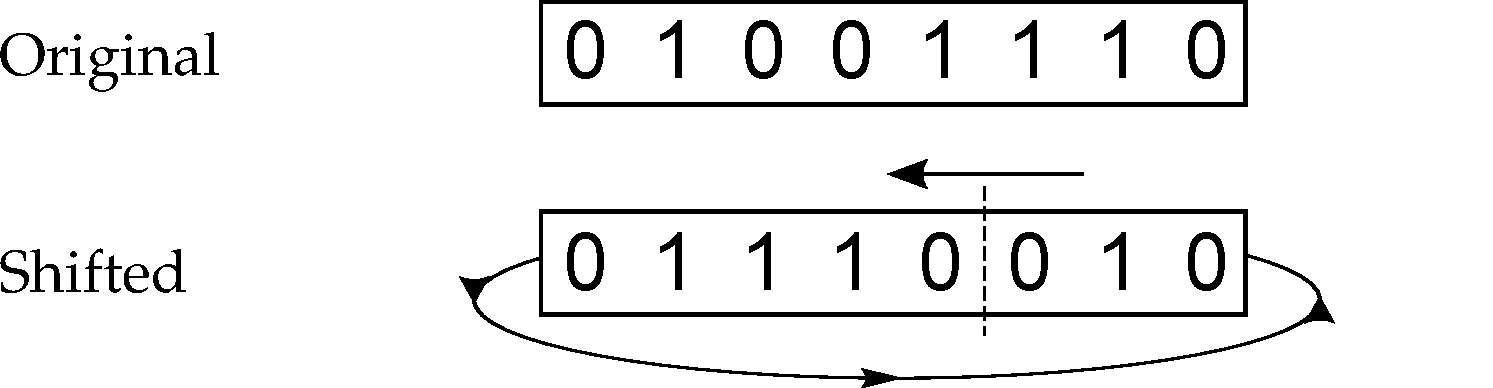
\includegraphics[width=4in]{ibcm/ibcm-shift-3.pdf}
\caption{A left rotation of 3}
\label{ibcm-shift-3}
\end{figure}

Note that the shift instructions uses bits 11-10 to specify the shift
operation.  The first bit specifies if it is a shift (0) or rotate
(1), and the second bit specifies if it is moving left (0) or right
(1).  This is shown in Table~\ref{IBCM-shift-instruction-values.tbl}.

\begin{table}[h]
\centering
\begin{tabular}{cccl}
\und{bit 11} & \und{bit 10} & & \und{operation} \\
0 & 0 & & shift left \\
0 & 1 & & shift right \\
1 & 0 & & rotate left \\
1 & 1 & & rotate right \\
\end{tabular}
\caption{IBCM shift/rotate bit values}
\label{IBCM-shift-instruction-values.tbl}
\end{table}

In addition, bits 3-0 of the shift instructions specify the ``shift
count''~-- that is, the number of bits positions that the data is to
be shifted (or rotated).

A left rotate of 3, which is what is shown in
Figure~\ref{ibcm-shift-3}, would have the opcode set to 2 (binary
0010), the shift/rotate bit set to 1, the left/right bit set to 0, and
the shift count set to 3.  The encoded instruction, in binary, is
shown in Figure~\ref{IBCM-right-rotate-of-3}.  Note that the
grayed-out part of the table are the bits whose value does not matter;
we set them to 0.

\begin{figure}[h!]
\centering
\begin{tabular}{|c|c|c|c|c|c} \cline{1-5}
0 0 1 0 & 1    &  0   &\cellcolor[gray]{0.8} 0 0 0 0 0 0 & 0 0 1 1 & =
0x2803 \\ \cline{1-5}
opcode  & rot. & left &\cellcolor[gray]{0.8} unused & shift \\
        & bit  & bit  &\cellcolor[gray]{0.8} bits   & count \\ \cline{1-5}
\end{tabular}
\caption{IBCM instruction for a right rotate of 3}
\label{IBCM-right-rotate-of-3} 
\end{figure}

As shown in the table, the hexadecimal encoding of the instruction is 0x2803.

\subsubsection{Other Instructions}

All other bit combinations in the left-most four bits either specify
an arithmetic instruction or a control instruction~-- similar to
assignment statements and {\tt goto}s in a high level language. The first four
bits are called the ``op'' field of the instruction; the value of this
field is often called the ``opcode''. The ``address'' portion of the
instruction generally specifies an address in memory where an operand
(variable) will be found.

There are 13 IBCM operations of this form~-- eight that manipulate
data and five that perform control. The data manipulation operations
all involve the ``accumulator'' and typically data from a memory
location is specified by the address portion of the instruction (the
{\tt not} and {\tt nop} instructions are the only two different ones).
The result of data manipulation operations is recorded in the
accumulator.  Thus, the ``add'' instruction forms the arithmetic sum
of the present contents of the accumulator with the contents of the
memory location specified by ``address'' and puts the result back into
the accumulator. Thus, it is similar to the primitive assignment
statement ``{\tt accumulator = accumulator + memory[address]}''.

The control instructions determine the next instruction to be
executed. The ``jump'' instruction, for example, causes the next
instruction executed to be the one at the location contained in its
address field. If you think of the address of a memory cell like a
label in a high level language, then jump is just ``{\tt goto
  address}''.

Two of the control instructions are conditional; they either cause a
change in the control flow or not, depending on the value of the
accumulator. The simplest of the control instruction is {\tt nop}; it
does nothing.

Table~\ref{IBCMopcodes.tbl} describes the function of each of these 13
IBCM instructions; both English and programming language-like
explanations are given for each instruction. In the latter, ``a'' is
the accumulator, ``addr'' is the values of the address portion of the
instruction, and ``mem[]'' is memory.

\begin{table}[h]
\centering
\begin{tabular}{llll}
\und{op} & \und{name} & \und{HLL-like meaning} & \und{English explanation} \\
3$_{16}$ & load  & a:= mem[addr]        & load accumulator from memory \\
4$_{16}$ & store & mem[addr] := a       & store accumulator into memory \\
5$_{16}$ & add   & a := a + mem[addr]   & add memory to accumulator \\
6$_{16}$ & sub   & a := a - mem[addr]   & subtract memory from accumulator \\
7$_{16}$ & and   & a := a \& mem[addr]  & logical 'and' memory into accumulator \\
8$_{16}$ & or    & a := a | mem[addr]   & logical 'or' memory into accumulator \\
9$_{16}$ & xor   & a := a $\oplus$ mem[addr] & logical 'xor' memory into accumulator \\
A$_{16}$ & not  & a := ~ a             & logical complement of accumulator \\
B$_{16}$ & nop   &                      & do nothing (no operation) \\
C$_{16}$ & jmp   & goto 'addr'          & jump to 'addr' \\
D$_{16}$ & jmpe  & if a = 0 goto addr   & jump to 'addr' if accumulator equals zero \\
E$_{16}$ & jmpl  & if a $<$ goto addr   & jump to 'addr' if accumulator less than zero \\
F$_{16}$ & brl   & branch and link      & jump (branch) to 'addr'; set accumulator to the value of the \\
         &       &                      & PC just before the jump (i.e., to the address following the brl \\
\end{tabular}
\caption{IBCM opcodes}
\label{IBCMopcodes.tbl}
\end{table}

A few words of additional explanation are necessary for some of these
operations, all of which are fairly standard for most computers.

\begin{enumerate}
\item Arithmetic operations may ``overflow'' or ``underflow''; that is,
the magnitude of the result may be larger than can be represented in
16 bits. The programmer is responsible for ensuring that this doesn't
happen.

\item The logical operations ({\tt and}, {\tt or}, {\tt xor}, and {\tt
    not}) perform bit-wise operations on the operands. The Boolean
  operations themselves are shown in Figure~\ref{IBCM-boolean-operations}.

\begin{figure}[h]
\centering
\begin{tabular}{ccccccc}
\begin{tabular}{c|c|c}
and & 0 & 1 \\ \hline \hline
0 & 0 & 0 \\ \hline
1 & 0 & 1 \\
\end{tabular}
& \hspace{0.5in} &
\begin{tabular}{c|c|c}
or & 0 & 1 \\ \hline \hline
0 & 0 & 1 \\ \hline
1 & 1 & 1 \\
\end{tabular}
& \hspace{0.5in} &
\begin{tabular}{c|c|c}
xor & 0 & 1 \\ \hline \hline
0 & 0 & 1 \\ \hline
1 & 1 & 0 \\
\end{tabular}
& \hspace{0.5in} &
\begin{tabular}{c|c}
not & \\ \hline \hline
0 & 1 \\ \hline
1 & 0 \\
\end{tabular}
\\
\end{tabular}
\caption{Boolean operation reference}
\label{IBCM-boolean-operations}
\end{figure}

\item The {\tt not} instruction only inverts the bits in the
  accumulator, and does not use a memory location; the 'address' part
  of the instrcution is ignored.

\item Likewise, the {\tt nop} instruction ignores the 'address' part
  of the instruction.

\item The branch and link instruction is used for subroutine calls, as
discussed later.

\end{enumerate}

\subsection{Other opcodes}

When writing an IBCM program, one will typically write out the IBCM
opcodes, such as {\tt add} and {\tt store}.  There are a few other
opcodes that are not listed above, but that will often appear in an
IBCM file:

\begin{itemlist}
\item {\tt dw} (for ``declare word''), for declaring variables
\item {\tt readH} and {\tt printH} are for reading or writing a
  hexadecimal value
\item {\tt readC} and {\tt printC} are for reading or writing an
  ASCII character
\item {\tt shiftL} and {\tt shiftR} are for the shifts
\item {\tt rotL} and {\tt rotR} are for the rotations
\end{itemlist}



\section{Sample Program}

Consider the IBCM program shown in
Listing~\ref{IBCM-sample-program.lst}.  This program does not compute
a useful result; that's coming next.  Instead, it is intended to show
how the IBCM works.

\begin{lstlisting}[caption=Sample IBCM program,backgroundcolor=\color{white},frame=trBL,linewidth=5.5in,xleftmargin=1.75in,label={IBCM-sample-program.lst}]
Address	Instruction	Opcode	Address
000	3000		load	000
001	5000		add	000
002	6001		sub	001
003	8003		or	003
004	a000		not	N/A
005	4000		store	000
006	f000		brl	000
\end{lstlisting}

Let's trace what this program does.  All the values below are in
hexadecimal.  All addresses are represented using three digits.

\begin{enumerate}

\item Address 000: Instruction value 3000.  Opcode 3 is a {\tt load},
  with an address of 000.  This will load the value in memory at
  address 000 into the accumulator.  The value in address 000 is
  3000~-- it is both the instruction being executed and the data being
  loaded.  The accumulator is now 3000.

\item Address 001: Instruction value 5000.  Opcode 5 is an {\tt add},
  with an address of 000.  This will add the value in memory at
  address 000 to the accumulator, and store the result in the
  accumulator.  The value in address 000 is 3000, so the result (and
  the new accumulator value) is 6000.

\item Address 002: Instruction value 6001.  Opcode 6 is a {\tt sub},
  with an address of 001.  This will subtract the value in memory at
  address 001 from the accumulator, and store the result in the
  accumulator.  The value at address 001 is 5000; 6000-5000=1000.
  Thus, the new accumulator value is 1000.

\item Address 003: Instruction value 8003.  Opcode 8 is an {\tt or},
  with an address of 003.  This will perform a bit-wise or'ing of the
  value in memory address 003 with the value in the accumulator, and
  store the result in the accumulator.  The value in address 003 is
  8003~-- again, we are using the same value for the instruction being
  executed and for the data being used.

To perform a bit-wise logical operation, write out the full bit values
for each of the operands, and perform the bit-wise operation (or, in
this case) on each of the bits in each column.

\begin{tabular}{ccccccccc}
& 0x8003 & = & 1000 & 0000 & 0000 & 0011 \\
$\lor$ & 0x1000 & = & 0001 & 0000 & 0000 & 0000 \\ \cline{1-7}
& & & 1001 & 0000 & 0000 & 0011 & = & 0x9003 \\
\end{tabular}

Thus, the value in the accumulator is 9003.

\item Address 004: Instruction value a000.  Opcode a is a {\tt not}
  operation.  This opcode ignores the address portion of the
  instruction, as the operation just inverts all the bits of the
  accumulator.  The bit value of the accumulator prior to the not
  operation is listed in the previous step.

\begin{tabular}{ccccccccc}
$\neg$ & 0x9003 & = & 1001 & 0000 & 0000 & 0011 \\ \cline{1-7}
& & & 0110 & 1111 & 1111 & 1100 & = & 0x6ffc \\
\end{tabular}

Thus, the value in the accumulator is 6ffc.

\item Address 005: Instruction value 4000.  Opcode 4 is a {\tt store}
  instruction, with an address of 000.  This will store the current
  value in the accumulator (6ffc) into memory at address 000.  The
  previous value in that spot (3000) is, of course, overwritten.

\item Address 006: Instruction value f000.  Opcode f is a {\tt brl}
  (branch and link) instruction, with address 000.  This will store
  the address of the next instruction (i.e., the address after 006, or
  007) in the accumulator, and jump to the specified address of 000.
  Thus, the value in the accumulator after this instruction is 0007,
  and the next instruction to be executed is address 000.

\item Address 000: Instruction value 6ffc.  Note that this value was
  written to memory two steps prior (the instruction at address 005),
  and control jumped to this instruction from the previous instruction
  (the instruction at address 006).  Opcode 6 is a {\tt sub}, with
  address ffc.  As all values in IBCM's memory are initialized to
  zero, the value in address ffc is thus zero.  Thus will subtract
  zero from the accumulator yielding the original value of 0007, which
  is what is stored in the accumulator after this instruction is
  executed.

\end{enumerate}

Program control will continue.  The next time the accumulator executes
the instruction at address 005 (instruction value 4000; opcode 4 is a
{\tt store}), the value written to address 000 will be 5ffc (opcode 5
is an {\tt add}).  The next time around, it will write 6ffc (opcode 6
is a {\tt sub}).  Thus, this program will loop forever, alternately
writing 6ffc and 5ffc to address 000 at the end of each loop.

One of the important points to note in the above program is that the
distinction between data and instructions is blurred.  The value 6ffc
is computed through a series of instructions, and then stored~-- as
data~-- at address 000.  But when the program control reaches that
point, the value of 6ffc~-- that was previously data~-- now becomes an
instruction.

We will see additional examples of using data as instructions, and
using instructions as data, in the example programs section, below.


\section{The IBCM Simulator/Debugger}

\begin{wrapfigure}{r}{0.5\textwidth}
\centering
\vspace{-0.15in}
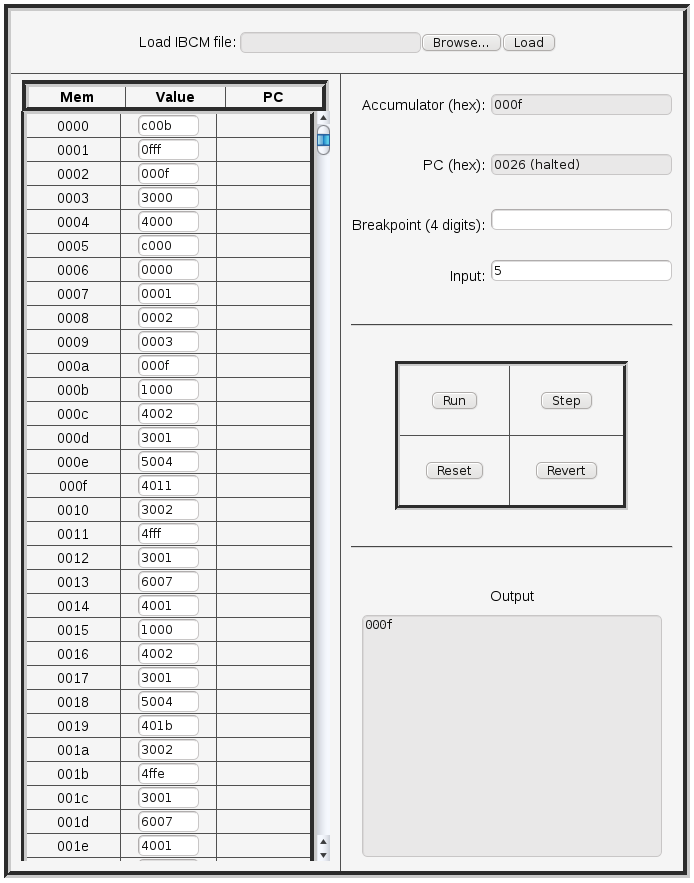
\includegraphics[width=3.25in]{ibcm/www-screen-shot.png}
\caption{Web-based IBCM interface}
\label{wwwinterface}
\vspace{-0.25in}
\end{wrapfigure}

To run an IBCM program, you can view the online simulator at
\url{http://libra.cs.virginia.edu/ibcm} \cite{ibcm-website}.  The
instructions listed in this section are also listed at that website.
An image of the online emulator is shown in Figure~\ref{wwwinterface}.

The simulator reads in text files, and proceeds to simulate the
result of an IBCM program execution.

To load a file, use the Browse button at the top of the simulator
page. Find the IBCM file, and click on the ``Load'' button. The format
of your program file is very rigid -- the first four characters of
each line are interpreted as a hexadecimal number. The number on the
first line is loaded into location zero, the next into location one
and so on. Characters after the first four on each line are ignored,
so you should use them to comment the code.  Blank lines are not
allowed, nor are lines that do not start with four hexadecimal digits
(i.e., no 'comment' lines).  An invalid file will either not load up
at all, or will load up gibberish.

The left side of the simulator lists all the memory locations (using
the hexadecimal address), the value in memory (if any), and the PC
(program counter) value. Note that any blank value field is
interpreted as'0000', as per the IBCM specification. When first
loaded, the simulator may uninitialized values blank to increase
readability.

The value column consists of a series of text boxes, which allow you
to directly edit the values in memory. The simulator will read the
current memory location from the appropriate text box when executing an
instruction. You can undo any edits by using the Revert button,
described below. The IBCM simulator does not check to ensure that your
entered values are valid~-- it is up to the user to do this. Note that
all hexadecimal values must be 4 digits (i.e. '0000', not '0'), or
else the simulator may not function correctly. Be sure to read the
section about crashing browsers and losing your work, below. There is
no way to save your edited work -- you will need to copy the changes
by hand. This is party due to a browser limitation, and partly due to
the fact that memory editing is meant to be a debugging tool, not a
means to write entire IBCM programs from scratch.

The 'PC' column lists the current value of the program counter. It can
have three values. Normally, it will have a left pointing arrow
('$<$-'), which indicates the next instruction that will be executed.
If the simulator is waiting for input, it will have a capital 'I' (for
Input) next to the input instruction that is currently awaiting a
value~-- and the ``Input'' text on the right side will blink. Lastly,
if the program has halted, then a capital 'H' (for Halt) will be
displayed next to the halt instruction that was executed.

On the right side, the values of the accumulator and program counter
are listed, both in hexadecimal notation. As mentioned above, the PC
field will also display, one the left side next to the hexadecimal
address, if the simulator is awaiting input or is halted. The Input
box is used to read in user input when a program requests it. When the
simulator is waiting for input, it will flash the 'Input' text. In
addition, the simulator will specify which type of input is being
requested: 'hex' or 'asc' for hexadecimal or ASCII input,
respectively. Note that for entering a hexadecimal value, you do not
need to enter all 4 digits: i.e., you can enter '12' instead of
'0012'. This is distinctly different that editing memory locations
(you have to enter all 4 digits for those). If you enter multiple
characters for ASCII input, it will only read in the first one.

Below this are four buttons. Two control execution: Run, which will
start a program executing, and Step, which will execute a single
instruction. Note that Run will execute until either a halt command is
reached, or until an input command is reached. The other two buttons
control the resetting of the IBCM program. The Reset button will reset
the PC and accumulator, in effect allowing the program to run again.
It will not, however, modify any memory locations. The Revert button
will do what a Reset does, but will also revert the memory locations
to what they were when the file was last loaded; it does not load the
file from disk again. Thus, if you have edited any of the memory
locations (or the IBCM program has modified them), then those changes
will be erased on a Revert, but not on a Reset. Note that a Revert
will not modify memory addresses outside the range that was loaded
(i.e. any 'blank' values).

Any output is displayed in the text area below these buttons. Each
output command prints the value (hexadecimal or ASCII character) on a
separate line.

A few notes:

\begin{itemize}

\item You will notice a slight delay when loading the simulator page.
  This is due to the fact that a number of scripts are run when the
  page loads (to initialize the memory table of 4096 elements, for
  example), and this takes a bit of time. How long this takes is
  determined by how fast a computer it is running on, as the scripts
  are run on the client side.

\item Upon entering input, hitting Enter is considered the same as
  hitting the Run button again. If you only want to execute a single
  instruction after an input, you must click on the Step button.

\item The simulator does minimal error checking with the input from
  the keyboard during program execution -- it is the user's
  responsibility to ensure that the input is properly formatted. The
  only error checking that is done is to ensure that a non-empty
  string was entered (if it was, then the simulator waits for more
  input).

\item Because of the limitations of threads running in web browsers,
  there is no way to terminate a program that is stuck in an infinite
  (or very long) loop -- the browser will not allow a polling
  (checking) to see if a Stop button was pressed, for example. Some
  browsers will pause the script after a minute or so of execution,
  and ask if the user wants to continue. Alternatively, you can close
  the web browser and restart. Note that this means if you have edited
  any of the memory locations, and your browser hangs or is restarted,
  you will lose any and all changes you have made to the memory
  locations!

\item The simulator page is a PHP script, which means that it will not
  work if you are viewing it as a local file (if the beginning of your
  URL is ``file://'' instead of ``http://''), or if the web server
  hosting this page does not have PHP installed (this latter
  restriction includes UVa's Collab web server).

\item Browser compatibility: It has been tested in Internet Explorer
  under Windows, Safari under Mac OS X, and Firefox under Windows, Mac
  OS X, and Ubuntu Linux. Note that the dispaly of the changing of the
  values as the simulation is run (the PC, memory values, etc.) will
  only work on some browser / operating system combinations (Firefox,
  in particular, works well for this). The other browsers will have
  the same end state after the program is run, but will not animate
  the execution of the IBCM program when 'Run' is pressed (the 'Step'
  command will still animate each step).

\item The format of your program file is very rigid~-- the first four
  characters of each line are interpreted as a hexadecimal number. The
  number on the first line is loaded into location zero, the next into
  location one and so on. Characters after the first four on each line
  are ignored, so you should use them to comment the code; example
  code will be discussed in class.

\item When you execute a {\tt halt}, the simulator will halt with the PC
  pointing at the {\tt halt}.

\end{itemize}

\section{Writing IBCM Programs}

\subsection{Complex control structures}

\begin{wrapfigure}{r}{0.31\textwidth}
\vspace{-0.1in}
\begin{lstlisting}[caption={\bf if} pseudo code,backgroundcolor=\color{white},frame=trBL,linewidth=2in,xleftmargin=0.25in,label={IBCM-pseudo-code-if.lst}]
if ( B == 0 )
  S1;
else
S2
\end{lstlisting}
\vspace{0.25in}
\end{wrapfigure}

The control structures that we are familiar with in higher level
languages can be implemented in IBCM, albeit with a bit more effort.
Consider a typical pseudo code if-then-else conditional shown in
Listing~\ref{IBCM-pseudo-code-if.lst} to the right.

\begin{wrapfigure}{r}{0.31\textwidth}
\vspace{-0.4in}
\begin{lstlisting}[backgroundcolor=\color{white},frame=trBL,linewidth=2in,xleftmargin=0.25in,label={IBCM-code-if.lst},caption={IBCM {\bf if} code}]
load B
jmpe S1
S2: ...
jmp done;
S1: ...
done: ...
\end{lstlisting}
\vspace{-0.25in}
\end{wrapfigure}

The IBCM code for this conditional is shown in
Listing~\ref{IBCM-code-if.lst}.  Because we do not know many of the
required addresses (of variable B, or where S1 and S2 start in
memory), we have chosen to leave it in assembly format (i.e., using
opcodes) rather than provide machine code.

If we wanted to compare B to a different value, such as 5, we would
have to load B into the accumulator, subtract 5 from that, and then
perform a {\tt jmpe} or {\tt jmpl}.  This is illustrated further
below, when discussing the while loop.

Presumably, the ellipses at labels S1 and S2 would have some set of
IBCM opcodes to execute.

\begin{wrapfigure}{r}{0.31\textwidth}
\vspace{0.1in}
\begin{lstlisting}[backgroundcolor=\color{white},frame=trBL,linewidth=2in,xleftmargin=0.25in,label={IBCM-pseudo-code-while.lst},caption={{\bf while} pseudo code}]
while ( B >= 5 )
  S;
\end{lstlisting}
\vspace{0.25in}
\end{wrapfigure}

Loops are also easily converted to IBCM.  Note that a {\tt for} loop
is just a {\tt while} loop, but with a statement performed before the
loop starts (the ``for init''), and a statement performed at the end
of each loop iteration (the ``for update'').  Consider a straight
forward while loop shown in Listing~\ref{IBCM-pseudo-code-while.lst}.

\begin{wrapfigure}{r}{0.31\textwidth}
\vspace{-0.7in}
\begin{lstlisting}[backgroundcolor=\color{white},frame=trBL,linewidth=2in,xleftmargin=0.25in,label={IBCM-code-while.lst},caption={IBCM {\bf while} code}]
loop: load B
sub five
jmpl done
S: ...
jmp loop
done: ...
\end{lstlisting}
\vspace{-0.5in}
\end{wrapfigure}

We cannot directly compare a variable to the value 5; we can only
compare it to zero via the {\tt jmpe} and {\tt jmpl} instructions.
Our IBCM code is shown in Listing~\ref{IBCM-code-while.lst}.

If $B<5$, then we want our loop to terminate.  If $B<5$, then $B-5<0$,
so we will execute a {\tt jmpl} to break out of the loop.  If $B=5$,
then $B-5=0$, and we will continue in the loop.

\subsection{General tips}

When writing IBCM programs, we recommend these steps:

\begin{enumerate}
\item Write the pseudo code first~-- or even actual code~-- to make
  sure your algorithm works as desired.  If you have a bug in the
  design of your algorithm, then you will never get your IBCM code to
  work.
\item Write the program using IBCM opcodes, so that it looks like
  assembly: {\tt add one}, {\tt store x}, etc.  Comment this clearly!
\item Trace this assembly code, by hand, from beginning to end.  It
  will be {\em far} easier to find a bug in your program in the
  assembly stage than in the hexadecimal code stage.
\item Finally, translate it to machine code, and run it in the
  simulator.
\end{enumerate}

We cannot stress enough how important it is to first make sure that
the algorithm works, then to write and trace the assembly versions of
the program.  Debugging hexadecimal machine code is not much fun.



\section{Example Programs}


We present a number of IBCM example programs to help you get
acquainted with the language.

\subsection{Summation}

\begin{wrapfigure}{r}{0.45\textwidth}
%\vspace{-0.25in}
\lstinputlisting[caption=C++ summation program,label={C++program1.lst},backgroundcolor=\color{white},frame=trBL,linewidth=3.2in,xleftmargin=0.25in,language=C++]{ibcm/summation.cpp}
\vspace{-0.25in}
\end{wrapfigure}

The first program will compute the sum of the integers 1 through $n$,
where $n$ is read from the keyboard; the resulting sum is printed to
the screen. The program then halts after printing the sum.  The C++
code for the program is shown in Listing~\ref{C++program1.lst}~-- this is
presented to help show the conversion to IBCM.

The IBCM program is shown in Listing~\ref{IBCM-summation-program.lst}.
Note that the only part of the program that the simulator reads in is
the first four characters on the line.  The rest of the line in the
text file is solely for comments.  The column headers shown in the
figure are heavily abbreviated to fit in the width of a column, but
are, in order: the actual 4 hexadecimal digit memory value, the
hexadecimal location (used for determining jump targets and variable
addresses), the label (used to refer to jump and variable targets),
the opcode (from Table~\ref{IBCMopcodes.tbl}), the target address (which
refers to a given label), and any English comments. Note that the
column headers would not be in the input file; only the IBCM
hexadecimal instructions.  They are included in the listing for
clarity.

\begin{figure}[h]
\lstinputlisting[caption=IBCM summation program,label={IBCM-summation-program.lst},backgroundcolor=\color{white},frame=trBL,linewidth=6in,xleftmargin=1in]{ibcm/summation.ibcm.txt}
\end{figure}

\subsection{Array usage}

\begin{wrapfigure}{r}{0.45\textwidth}
%\vspace{-0.2in}
\begin{lstlisting}[caption=Array index pseudo code,label={array-index-pseudo-code.lst},backgroundcolor=\color{white},frame=trBL,linewidth=3.2in,xleftmargin=0.25in]
read A
read N
s = 0
i = 0
while (i < N)
	s += a[i]
	i += 1
print s;
\end{lstlisting}
\vspace{-0.4in}
\end{wrapfigure}

For this program, we will compute the sum of the elements of an array,
print this sum on the screen, and then halt.  Note that the array is
just a series of sequential spots in memory; it could be part of the
program itself, or a series of data values after the program itself.
The address of the first element of the array and the size of the
array are to be read from the keyboard.

The pseudo code for this program is shown in
Listing~\ref{array-index-pseudo-code.lst}.  C++ does not easily allow
for reading in an array address (while technically possible, it is not
very practical), so a C++ version of this program is not as useful as
a pseudo code version.

The IBCM code is shown in Listing~\ref{IBCM-array-index-program.lst}.

\begin{figure}[h!]
\lstinputlisting[caption=IBCM array index program,label={IBCM-array-index-program.lst},backgroundcolor=\color{white},frame=trBL,linewidth=6.8in,xleftmargin=0.25in]{ibcm/array-index.ibcm.txt}
\end{figure}

A quick note before the full analysis.  Notice that addresses 08
and 09 are blank~-- this was done to leave space for additional
variables.  If one has to add a variable into the program later,
shifting all of the successive instructions down is a frustrating
task, as all the addresses (of the jump targets, etc.)  need to be
shifted as well. So we left a few blank lines in case we needed
additional variables later on.

The challenging part of this program is the array subscripting.  In
our pseudo code~-- and in most programming languages~-- we use a syntax
such as {\tt a[i]}.  But the IBCM does not have any array subscripting
instruction~-- indeed, it cannot, as that requires two values (the
array base and the index). Thus, we have to {\em build} the
instruction to execute.

Our goal is to load the current sum (of the array elements processed
so far) into the accumulator, execute the instruction to add the
current {\tt a[i]} to the accumulator, and store that back into the
sum variable.  This is done in instructions 19, 1a, and 1b:
instruction 19 loads the current sum into the accumulator, instruction
1a is our special instruction that adds {\tt a[i]} to the accumulator
(how this works is next), and instruction 1b stores the updated result
back into the sum variable (address 002).

Thus, we want to create an instruction that will add a given {\tt
  a[i]} to the accumulator.  So we know it will be an add instruction
(opcode of 5).  The address that we want to add to the accumulator is
the array base plus the index.

For example, if the array starts at address 100, and we are trying to
add the value at index 5 of the array, our instruction would have
opcode of 5 (an add instruction), and address 105 (100 for the array
start plus 5 for the current index).  Thus, our instruction would be
5105.

To create this during the program execution, we start with 5000, which
sets the opcode of the instruction to the correct value for an add
instruction.  This is done in instruction 15, which is a load of the
{\tt adit} variable (address 007), which has value 5000.  To this
value of 5000 we add the array base (instruction 16) and then the
index (instruction 17).  Instruction 18 then stores that instruction
at the appropriate address (address 1a), overwriting the nop that is
there with our updated instruction.  Once the current sum is loaded
(instruction 19), our custom instruction is executed (instruction 1a),
followed by the sum being stored back into memory (instruction 1b).


\subsection{Recursive multiplication}

The next program computes the product of two numbers, $x$ and $y$,
through a recursive multiplication subroutine that uses only addition.
Both $x$ and $y$ are read from the keyboard, and the resulting product
is printed to the screen. The IBCM version is just over 100 lines of
opcodes.

\begin{wrapfigure}{r}{0.45\textwidth}
\vspace{-0.15in}
\lstinputlisting[backgroundcolor=\color{white},frame=trBL,linewidth=3in,xleftmargin=0.25in,language=C++,label={C++-multiplication-program.lst},caption={C++ multiplication program}]{ibcm/mult.cpp}
\vspace{-0.4in}
\end{wrapfigure}

The C++ code for the multiplication program can be seen in
Listing~\ref{C++-multiplication-program.lst}.  We did not create a
tail recursive {\tt multiply()} routine, as the IBCM compiler and
language is (intentionally) far too simple to optimize for tail
recursion.

This IBCM program creates a stack similar to x86: the stack starts at
the end of addressable memory, and grows downward.  An activation
record is created for each recursive call, which consists of the two
parameters and the return address~-- other fields typically in an
activation record (e.g., backup of registers) are not necessary in
IBCM.  The {\tt brl} instruction was used to allow for subroutine
calls~-- the return address is saved in the accumulator, and is stored
on the stack immediately upon subroutine activation.  We were able to
run the program with the second parameter (which is decremented in
each recursive call) set as high as 1,243 (0x4db), beyond which point
IBCM runs out of available memory for the stack.

This recursive multiplication program is beyond what we would expect
of a student to be able to program after a one-week introduction to
IBCM.  However, it is very illustrative of two important points about
IBCM.  One is that complex functionalities (such as multiplication)
can be achieved by using only the simple capabilities available in
IBCM (such as addition).  The other is that subroutines are fully
realizable in IBCM.

This program is shown in
Listings~\ref{IBCM-multiplication-program-pt1.lst} and
\ref{IBCM-multiplication-program-pt2.lst}.  Note that the only part of
the program that the simulators read in is the first four characters
on the line.  The rest of the line in the text file is solely for
comments.  The column headers and extra blank lines for comments are
shown in the diagram for clarity, but would not be included in the
IBCM source code file.

\begin{figure}
\lstinputlisting[caption={IBCM multiplcation program, part 1},label={IBCM-multiplication-program-pt1.lst},backgroundcolor=\color{white},frame=trBL,linewidth=7.05in,xleftmargin=0.15in]{ibcm/multiplication-pt1.ibcm.txt}
\end{figure}

\begin{figure}
\lstinputlisting[caption={IBCM multiplcation program, part 2},label={IBCM-multiplication-program-pt2.lst},backgroundcolor=\color{white},frame=trBL,linewidth=7.05in,xleftmargin=0.15in]{ibcm/multiplication-pt2.ibcm.txt}
\end{figure}

\section{Turing Completeness}

We were conflicted as to how much to discuss about Turing completeness
in this chapter.  IBCM is similar to a Random Access Stored Program
(RASP) machine \cite{wikipedia:rasp}, which is itself Turing complete,
so it is perhaps not surprising that IBCM is also Turing complete.
However, we felt that breaking down a complex task (a Turing machine
simulator) and programming it into IBCM was a worthwhile task to
discuss, as it emphasizes a primary design goal of IBCM~-- that
you can take any algorithm and write it in IBCM.

\begin{figure}[h]
\centering
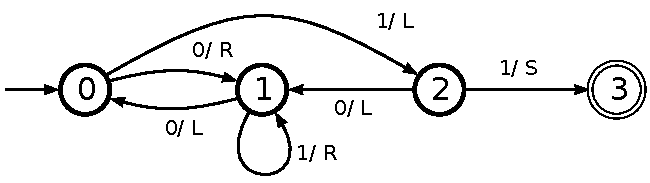
\includegraphics[width=4in]{ibcm/ibcm-automata.pdf}
\caption{Four state Busy Beaver automaton}
\label{BusyBeaverAutomaton}
\end{figure}

Obviously, no physical computer with a finite amount of memory can be
truly Turing complete.  Thus, we will instead show that the IBCM
computational model is Turing complete.

We define the {\em IBCM computational model} as the same IBCM computer
defined above, but allowing any sized integer to be held in a single
memory location, as well as having an infinite amount of memory.
Thus, other fields that make up part of a given instruction, such as
the 'address' or 'count' fields (see
Figure~\ref{IBCMInstructionFormat}), can also hold any size integer.

Given this model of computation, we will show how to simulate a Turing
machine in IBCM.  Hopcroft and Ullman \cite{HopcroftAndUllman} define
a Turing machine as a 7-tuple $M=\langle
Q,\Gamma,b,\Sigma,\delta,q_0,F \rangle$ where:

\begin{itemlist}
\item $Q$ is a finite set of states
\item $\Gamma$ is the finite set of allowable tape symbols
\item $b \in \Gamma$ is the blank symbol
\item $\Sigma \subseteq \Gamma \setminus {b}$ is the set of input symbols
\item $\delta : Q \times \Gamma \rightarrow Q \times \Gamma \times \{L,R\}$ is the transition function
\item $q_0 \in Q$ is the initial state
\item $F \subseteq Q$ is the set of final states
\end{itemlist}

We will make two modifications to the above definition, to allow for
ease of implementation in IBCM.  We will allow a no-shift transition
of $S$ (in addition to $L$ and $R$), which will not move the tape.
The Turing machine programs allowed by the no-shift are equivalent to
the ones described above \cite{wikipedia:turingmachine}. Furthermore,
we will define $f$, a single final state, which all states in $F$ move
to on a no-shift transition.

To represent the transition functions in IBCM, we will represent state
$q \in Q$ and symbol $\Sigma \in \Gamma$ each as a (16-bit) word in
IBCM.  Thus, states and symbols will be a single integer each.  While
this limits the number of states (and symbols) to $2^{16}=65,536$ in
our IBCM implementation, it is not limited in the formal IBCM
computational model.  Thus, one can encode any amount of states,
symbols, and transition functions into IBCM's memory.

To simulate a Turing machine, we will define an arbitrary memory
location to represent the current state of the Turing machine, and
another arbitrary memory location to contain the current address of
the head of the tape.  The transition function quintuples, $\delta$,
will start at a specific (but arbitrary) memory address, take up five
words each, and will contain the five parts listed above
$(Q,\Gamma,Q,\Gamma,\{L,R,S\})$.  The tape itself will start at
different arbitrary memory location.  Furthermore, we define a initial
state $q_0$ and a (single) final state $f$.  The blank symbol $b$ will
be an arbitrary value, such as -1 (0xffff in 16-bit 2's complement
integer).

Any Turing machine that requires a significant amount of tape will
need to be a one-way tape Turing machine, as the program code and
state transitions will lie at a lower address than the initial head
position.  Thus, only a finite amount of tape space is available in
the lower memory address direction.  The particular automaton example
that we provide, below, uses a two-way tape, but that is because we
know the finite amount of tape space necessary.  Note that one-way
tape Turing machines are equivalent in computational power to two-way
tape Turing machines \cite{HopcroftAndUllman}.

What is needed, then, is an IBCM program that will iterate through the
following steps:

\begin{itemlist}
\item Read the current state $s$, initially set to the start state.
  If the current state is the (single) final state, then exit.
\item Read the current head position.
\item Read the current input symbol $t$ at the head position
\item Search the list of transition functions until the appropriate
  one is found, based on the current state $s$ and the input symbol
  $t$.
\item Perform the action specified in the transition function by
  updating the state $s$, writing the specified symbol to the tape
  position, and then moving the tape left or right (or, on an $S$, not
  at all).
\end{itemlist}

We have developed such a program, described here.  The full listing of
the program is available online \cite{ibcm-website}.  The program
consists of 67 IBCM commands, and 15 variables~-- note that numeric
constants are considered variables in an IBCM program.  This program
only used half of the instructions: {\tt halt}, {\tt load}, {\tt
  store}, {\tt add}, {\tt sub}, {\tt nop}, {\tt jmp}, and {\tt jmpe}.

To test the Turing machine, we choose a four state Busy Beaver
automaton, which is described in more detail in the Wikipedia page on
Turing machine examples \cite{wikipedia:turingmachineexamples}.  The
Mea\-ly machine finite automaton is shown in
Figure~\ref{BusyBeaverAutomaton}.  For each transition, the input
symbol (0 or 1) is shown, along with the tape direction to move ($L$,
$R$, or $S$).  Note that in this automaton, upon each transition a 1
is written to the output tape; this is not shown in the figure to
improve clarity.  Also recall that the $S$
transition means to not move the tape, and is used only on the
transition to the final state.

Our implementation can utilize a two-way tape, although the tape in
one direction is finite.  We define memory address 1 as the current
state variable, and address 2 to store the location of the current
head position.  The transitions start at address 0x060, as our program
takes up 82 (or 0x052) instructions.  The states are numbered as per
the diagram in Figure~\ref{BusyBeaverAutomaton}, with 0 being the
initial state and 3 being the final state.  The program has constants
that specify both the initial and final states of the automaton.

% automaton figure goes here

The encoding of the automaton shown in
Figure~\ref{BusyBeaverAutomaton} is very straightforward.  The
transition from 2 to 1, executed on an input symbol of 0, will print 1
to the tape and then move the tape to the left.  The quintuple to be
encoded is $Q \times \Gamma \rightarrow Q \times \Gamma \times
\{L,R,S\}$.  The respective values for this transition are
$2,0,1,1,0$; we map the integer values $\{0,1,2\}$ to, respectively,
the transition directions $\{L,R,S\}$.


\section{Emulating IBCM in C++}

How might one write software to emulate an IBCM machine in C++?  A
switch statement with 16 cases, perhaps.  But how to decode the
instructions?

Let's assume we had to write a C++ program that could extract the
parts of an IBCM instruction.  How to do it?  Assume the instruction
is in an {\tt unsigned int x}.  One way to decode it is shown in
Listing~\ref{IBCM-decoding-instruction.lst}

\lstinputlisting[language=C++,backgroundcolor=\color{white},frame=trBL,linewidth=5.5in,xleftmargin=1.5in,label={IBCM-decoding-instruction.lst},caption={Decoding an IBCM instruction in C++}]{ibcm/emulating1.cpp}

What about encoding?  Assuming we have (unsigned ints) opcode,
ioshiftop and shiftcount, the decoding is shown in Listing~\ref{IBCM-encoding-instruction.lst}

\lstinputlisting[language=C++,backgroundcolor=\color{white},frame=trBL,linewidth=6.85in,xleftmargin=0.1in,label={IBCM-encoding-instruction.lst},caption={Encoding an IBCM instruction in C++}]{ibcm/emulating2.cpp}

This ends up being a rather frustrating program to write.  If the
instruction set being dealt with is more complicated than IBCM, as is
the case with x86 or MIPS instructions, then the above is very
difficult to do without any errors.

Listing~\ref{IBCM-encoding-data-structure.lst} shows a data structure
to make it easier.  While the IBCM is a big-Endian machine, the
following code may be running on a big or little-Endian machine.  The
{\tt BIG\_ENDIAN} and {\tt LITTLE\_ENDIAN} defines specify the
Endianness of the host machine.

\begin{figure}[h!]
\lstinputlisting[language=C++,backgroundcolor=\color{white},frame=trBL,linewidth=6.25in,xleftmargin=1in,label={IBCM-encoding-data-structure.lst},caption={C++ data structure to ease IBCM instruction encoding}]{ibcm/emulating3.cpp}
\end{figure}

We would use the data structure as shown in Listing~\ref{IBCM-encoding-data-structure-usage.lst}.

\begin{figure}[h!]
\lstinputlisting[language=C++,backgroundcolor=\color{white},frame=trBL,linewidth=6.25in,xleftmargin=1in,label={IBCM-encoding-data-structure-usage.lst},caption={Using the C++ data structure to encode IBCM instructions}]{ibcm/emulating4.cpp}
\end{figure}

\section{Pedagogy}

IBCM was originally developed at the University of Virginia to
complement our CS 3 course entitled {\em Program and Data
  Representation}, which is still taught today.  This course shows how
one represents both data and program code from high levels~-- such as
abstract data types~-- all the way down to the lowest (software)
level, which is the IBCM machine language.

IBCM allows students to easily make the mental connection between
assembly opcodes and the machine language that they get translated
into.  At the University of Virginia, we follow the presentation of
IBCM with a two-week introduction to x86 assembly language.  This
allows students to understand both machine language, as well as a
modern processor's assembly language (we use Intel x86), without
having to delve into the details of x86 machine language.

A specific design decision with IBCM was to include only basic
operations~-- for example, multiplication and division are not
included, but can be replicated by using repeated addition or
subtraction.  We wanted students to see that any program, no matter
how complicated, can be broken down into very simple instructions.
Indeed, this is the point of the concept of Turing machines, but they
are often not taught when students are first seeing machine language.

Students are exposed to a number of concepts during the IBCM module
that they often have not seen previously.  They become aware that in
both assembly language and machine language, data is untyped, and the
operations on the data determine the type~-- this is quite different
than the typed high-level programming languages to which they are
accustomed.  By this point in our course, students have been exposed
to how a 32-bit value can be interpreted either as a two's-complement
signed integer or an IEEE 754 floating point number.

Another concept taught through IBCM is self-modifying programs.  A
non-trivial IBCM program requires arithmetic on instructions~-- in
fact, only the first example program shown in
Listing~\ref{IBCM-summation-program.lst} did not use this feature.  Array indexing,
for example, requires starting with a {\tt load} or {\tt add}
instruction, and adding to that value both the base address of the
array and the current index.  This value is then stored in a memory
address which is shortly thereafter executed.  The second example
program provided to the students uses this feature.  While many
systems explicitly try to prevent self-modifying code, as that is an
exploit used by a significant amount of malware, it is still a concept
that the students should be familiar with.

The development of self-modifying IBCM programs leads to another
pedagogical goal of the course: the interplay between data and program
code.  Indeed, there is little difference between data and program
code, other than the values (obviously), and how it is interpreted
(and, in modern systems, what segment of an executable in which the
data is found).  This concept seems trivial to instructors, but is one
that students who have only programmed using high-level languages are
often unfamiliar with.

What IBCM does not teach, of course, is how binary machine
language instructions are executed on the processor.  Understanding of
this material is typically beyond all but senior-level undergraduate
courses; at many institutions, this is also outside the
standard computing curriculum.

\subsection{Materials Available}

We have developed and made available a wide range of materials for the
purpose of teaching the IBCM module.  The materials are all released
under various Creative Commons licenses.  They are available online
\cite{ibcm-website}, and consist of:

\begin{itemlist}
\item A PowerPoint slide set to introduce the concepts during a
  lecture-based course.  This 42 slide set takes about three 50-minute
  lectures to present.
\item A {\em Principles of Operation} document, which describes the
  IBCM computer and language, and how to write a program.
  It covers similar content to the lecture slides.
\item Sample programs, one of which was shown in
  Listing~\ref{IBCM-summation-program.lst}, above.  We also provide sample programs
  on array indexing, for example.  All the programs mentioned in this
  article are available online.
\item Sample student assignments, which require students to
  write additional IBCM programs beyond the sample programs provided.
  One of the assignments is to write a quine, or an IBCM program that
  will print itself out~-- the smallest quine produced is nine IBCM
  commands.
\item An online PHP/Javascript simulator, which is the primary way that
  the students program in IBCM.  This is shown above in
  Figure~\ref{wwwinterface}.  The PHP is used to allow loading of an
  IBCM program from a text file; the Javascript implements the IBCM
  simulator in the browser itself.  The simulator works across all
  major browsers on all major operating systems.
\item A C++-based command-line program, which can both compile and
  execute IBCM programs.  Not surprisingly, this is much faster than
  the online simulator.  This is particularly useful for automated
  compilation and execution of IBCM programs for grading, or for very
  long programs, such as the recursive multiply routine described
  above.
\end{itemlist}

Furthermore, a GUI-based tool for executing IBCM programs is available
separately \cite{jwelsh-ibcm}.
This tool allows for drag-and-drop loading of IBCM files into the
GUI, and compiles natively for each operating system.

% web interface image goes here

We very specifically have not developed an IBCM assembler, which would
take in the opcodes in an assembly language format and output
hexadecimal machine code.  The purpose of IBCM is to teach the
students machine language; given an IBCM assembler, this module ends
up being just a different assembly language for the students to learn.

\subsection{Related Work}

We are certainly not the first to propose a simplified machine
language as a pedagogical tool.  Andrew Tanenbaum's original 1984
text, {\em Structured Computer Organization}~-- now in its 5th
edition~-- presents the Mic-1 micro architecture and the Mac-1 machine
language \cite{538160}.  Indeed, the Mac-1 machine language has many
similarities with IBCM~-- this is not surprising, as there are many
common elements that must be present in all small instruction set
machine languages.  Further research in that decade presented
implementations of those languages \cite{54147,152757}.  The Mic-1
simulator, which is focused on assembly language, is available online
\cite{mic-1-website}.  Simulators for the Mac-1 machine language do
exist, but seem to be independently developed, and without a modern
set of implementation software.

A number of high quality simulators exist at the assembly level.
Pep/8 \cite{warford:2010:PMT:1734263.1734389,warford2009computer} is a
16-bit CISC architecture designed to teach assembly language concepts.
While it can be used for machine language~-- and can trace program
execution at the machine language level~-- the primary pedagogical
design is at the assembly language level. Another example is SPIM,
which is a full featured MIPS 32-bit simulator \cite{spim-website}.

Additional research on machine language simulators has often focused
on the register transfer level \cite{107081}, or is restricted to a
single client operating system \cite{199795}.

More recent research by Stone has focused on a similar machine
language implementation \cite{1189166}.  Although developed
independently, our research can be seen as an extension of Stone's, as
we add a number of additional aspects: significant pedagogical tools,
a fully downloadable package so this system can be used in any course,
a proof of Turing completeness, and a discussion of pedagogical
concerns.  

We are not aware of any machine language simulators that are available
with the set of modern tools that we present with IBCM.


\subsection{Results}

At the University of Virginia, this module is taught about half-way
through our CS3 course, which is where we teach data structures.  Our
CS1 and CS2 course are both in Java.  At this point in the CS3 course,
the students have learned to implement a number of data structures in
C++.  We introduce machine language using IBCM for one week, follow
that with two weeks of assembly programming (x86), and then return to
C++ for the remainder of the semester.  The lectures used to teach
IBCM typically take three 50-minute class periods.  This is followed
by an IBCM lab the following week.  All of the lecture slides and labs
are available online~\cite{ibcm-website}.

We have taught machine language using IBCM in our CS3 class for over a
decade here at the University of Virginia.  Over the years, student
reactions to IBCM have varied greatly.  With the usage of the modern
tool set presented in this article, those reactions have generally
been positive, as shown below While they often do not like being
constrained to such a limited set of instructions, they see the
purpose of learning machine language, and generally enjoy the IBCM
assignments.  We have found that the quality of the software tools is
directly related to student perception of IBCM~-- in the past, when
our IBCM simulator was less refined, student reaction was
significantly more negative.

Objective comparison with other programming languages, including
assembly language, are difficult due to the vast differences between
both the capabilities and the required learning curve.  We have
instead focused on subjective assessment.  In the most recent semester
in which IBCM was used (fall of 2010), six questions were asked of the
students.  All questions were asked on a Likert scale, where 1 means
strongly agree, 2 is agree, 3 is neutral, 4 is disagree, and 5 is
strongly disagree.  For all the questions, $n=89$.

The first two questions focused on how much the students felt they
learned from the IBCM module.  The middle two questions focused on the
ease of use and enjoyability.  And the last two questions focused on
how worthwhile this module was, both for this course and future courses.
The results are shown in Table~\ref{IBCM-survey-results.tbl}.

\begin{table}[h]
\centering
\begin{tabular}{|p{5in}|c|c|}  \hline
\bf Question & \bf Avg & \bf Stdev \\ \hline \hline
IBCM increased my understanding of the basics of machine language &
1.67 & 0.58 \\ \hline
IBCM increased my understanding of how computers work at a low level &
1.89 & 0.65 \\ \hline
IBCM was easy to use, once I got the hang of programming in it & 1.92
& 0.88 \\ \hline
I enjoyed learning IBCM & 2.01 & 0.98 \\ \hline
Considering what was taught, IBCM was a worthwhile module to have in
this course & 1.75 & 0.68 \\ \hline
IBCM should be used in future iterations of this course & 1.76 & 0.72
\\ \hline
\end{tabular}
\caption{IBCM survey results}
\label{IBCM-survey-results.tbl}
\end{table}

The results clearly show that the module was generally well received.
The lowest score, enjoyment of learning IBCM, still was in the 'agree'
category.

\section{Conclusions}

We have used IBCM for over a decade at the University of
Virginia in our CS3
class.  During that time, we have refined it into the pedagogical tool
presented here.  With the set of current pedagogical tools provided,
we have found it to be an effective means of teaching the basic
concepts of machine language without having to go into the complexity
of modern machine languages that is beyond the scope of a lower-level
undergraduate course.  All of the necessary materials are available
online for adoption at other institutions.
